\scanpage{8}
\mspage{c}
Nous nous intéressons maintenant à des propriétés de stabilité \deleted{de la}\inserted{pour les} sous catégories \(\underline{\mathrm{Hom}}(B^o,A)\) de \((A\times B)^\wedge\), et \(A\) de \(A^\wedge\). Le foncteur \(p_{B*}\;(=(\Gamma_B)\circ)\) applique \deleted{\((A\times B)'\)} \(\underline{\mathrm{Hom}}(B^o,A)\) dans \(A\), dès que \(B\) admet un objet final \(e_B\) (car il s'identifie alors à \(\unsure{\Gamma|E}_{e_B}''\)). Donc on trouve
\diagram{\begin{tikzcd}
&\underline{\mathrm{Hom}}(B^o,A)\arrow[dl]\arrow[dr,"(\Gamma_A)\circ"]&\\
A^{\deleted{\unsure{\wedge}}}\arrow[dr,"\Gamma_A"']&&B^\wedge=\underline{\mathrm{Hom}}(B^o,(\mathrm{Ens}))\arrow[dl,"\Gamma_B"]\\
&{}&
\end{tikzcd}}
\uline{NB} (On pense au cas où \(B=\Delta\) p. ex (cat des simplexes-types) donc \(\underline{\mathrm{Hom}}(B^o,A)=sA\) objets simpliciaux de \(A\).
\deleted{\unsure{Je ne sais pas}}

\deleted{On} On s'intéresse \deleted{\unsure{au}} au cas où \(\underline{\mathrm{Hom}}(B^o,A)\) est stable par
\[\underline{\mathrm{Hom}}(p_A^*(M),X)\overset{\mathrm{def}}=X^M\qquad\text{pour }\forall\ M\in\mathrm{Ob}B^\wedge.\]
\margin{(\unsure{ou nous rest. aux ensembles de fins homot.})}
(alors que \(\underline{\mathrm{Hom}}(B^o,A)\) ne contient pas néc\unsure{\({}^{\mathrm{t}}\)} les \(p_A^*(M)\)\ldots\(^{*}\))

Il suffit que \(A\) soit stable par \(\varprojlim\) des types requis pour représenter \(M\) \inserted{comme \(\varinjlim\)} en termes de foncteurs représentables.
\margin{\figure{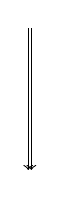
\begin{tikzpicture}\draw[->] (0,1.8)--(0,0);\draw[->] (.04,1.8)--(.04,0);\end{tikzpicture}}}
Noter qu'alors aussi
\[
\begin{aligned}
\underline{\mathrm{Hom}}_B(X,Y^M)&\simeq p_{A*}\underbrace{\underline{\mathrm{Hom}}(X,\underline{\mathrm{Hom}}(p_A^*(M),Y))}\\
&\simeq p_{A*}(\underline{\mathrm{Hom}}(X\times p_A^*(M),Y))\\
&\simeq\mathrm{Hom}_B(X\times p_A^*(M),Y).
\end{aligned}
\]
\margin{\(^{*}\) Pour \unsure{construire|avoir} \(p_A^*(M)\), il faudrait que \(\forall b\in\unsure{M|B}\) \inserted{\unsure{(pour b donné)}}, le foncteur \uline{constant} sur \(A\) de valeur \(M(b)\) soit représentable. Mais cela signifie que \(M(b)\) est réduit à \unsure{un élém.|un élément} et \(A\) a \unsure{objt} final. Donc \unsure{OK ssi} \(M\) objet final de \(\widehat B\), et \(A\) admet objet final !!}
\mspage{7}
